\documentclass[aspectratio=169]{beamer}

\usetheme{Boadilla}
\usefonttheme{professionalfonts}
\setbeamertemplate{navigation symbols}{}
\setbeamertemplate{itemize items}[circle]
\setbeamertemplate{enumerate items}[default]
\setbeamertemplate{headline}{}

\usepackage[utf8]{inputenc}
\usepackage[T1]{fontenc}
\usepackage{lmodern}
\usepackage{amsmath}
\usepackage{booktabs}
\usepackage{tabularx}
\usepackage{array}
\usepackage{hyperref}
\usepackage[strings]{underscore}
\usepackage{listings}
\usepackage{tikz}
\usetikzlibrary{arrows.meta,positioning,fit,calc,shapes.geometric}
\usepackage{xcolor}

\definecolor{courseblue}{HTML}{12355B}
\definecolor{coursegold}{HTML}{C98A2E}
\definecolor{courseice}{HTML}{EEF3F8}
\definecolor{coursegreen}{HTML}{2F6B4F}
\definecolor{coursegray}{HTML}{4B5563}
\definecolor{codebg}{HTML}{F7F9FC}
\definecolor{codecomment}{HTML}{5E6C84}
\definecolor{codestring}{HTML}{0B6E4F}

\setbeamercolor{palette primary}{bg=courseblue,fg=white}
\setbeamercolor{palette secondary}{bg=coursegold,fg=white}
\setbeamercolor{palette tertiary}{bg=courseblue,fg=white}
\setbeamercolor{palette quaternary}{bg=coursegold,fg=white}
\setbeamercolor{structure}{fg=courseblue}
\setbeamercolor{frametitle}{bg=courseice,fg=courseblue}
\setbeamercolor{title}{fg=courseblue}
\setbeamercolor{block title}{bg=courseblue,fg=white}
\setbeamercolor{block body}{bg=courseice,fg=black}
\setbeamercolor{normal text}{fg=black,bg=white}
\setbeamercolor{alerted text}{fg=coursegold}

\setbeamerfont{footline}{size=\scriptsize}

\setbeamertemplate{footline}{
  \leavevmode
  \hbox{
    \begin{beamercolorbox}[wd=.33\paperwidth,ht=2.8ex,dp=1.2ex,leftskip=0.8em]{palette primary}%
      University of Trieste
    \end{beamercolorbox}%
    \begin{beamercolorbox}[wd=.49\paperwidth,ht=2.8ex,dp=1.2ex,center]{palette tertiary}%
      \coursename{} \textbar{} \coursecode
    \end{beamercolorbox}%
    \begin{beamercolorbox}[wd=.18\paperwidth,ht=2.8ex,dp=1.2ex,rightskip=0.8em plus1fil]{palette secondary}%
      \insertframenumber{} / \inserttotalframenumber
    \end{beamercolorbox}%
  }
}

\hypersetup{
  colorlinks=true,
  linkcolor=courseblue,
  urlcolor=coursegreen
}

\lstdefinestyle{coursepython}{
  language=Python,
  basicstyle=\ttfamily\footnotesize,
  keywordstyle=\color{courseblue}\bfseries,
  commentstyle=\color{codecomment}\itshape,
  stringstyle=\color{codestring},
  showstringspaces=false,
  columns=fullflexible,
  keepspaces=true,
  frame=single,
  framerule=0.6pt,
  rulecolor=\color{courseblue},
  backgroundcolor=\color{codebg},
  xleftmargin=0.4em,
  xrightmargin=0.4em,
  aboveskip=0.4em,
  belowskip=0.2em
}

\newcommand{\coursename}{Data-driven Systems Engineering}
\newcommand{\coursecode}{440MI / 305SM}
\newcommand{\coursefooter}{}

\newcommand{\learninggoals}[1]{
  \begin{block}{Learning goals}
  #1
  \end{block}
}

\newcommand{\repoactivity}[1]{
  \begin{block}{Repo activity}
  #1
  \end{block}
}

\newcommand{\readinglist}[1]{
  \begin{block}{Papers and materials}
  {\footnotesize #1}
  \end{block}
}

\newcommand{\coursecontextframe}[5]{
  \begin{frame}{Course Map and Running Cases}
  \centering
  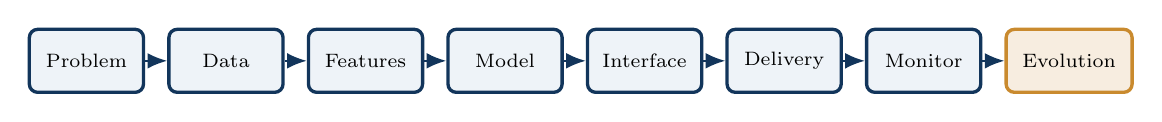
\begin{tikzpicture}[node distance=0.28cm]
  \node[flowbox, minimum width=1.45cm, minimum height=0.8cm] (problem) {\scriptsize Problem};
  \node[flowbox, minimum width=1.45cm, minimum height=0.8cm, right=of problem] (data) {\scriptsize Data};
  \node[flowbox, minimum width=1.45cm, minimum height=0.8cm, right=of data] (features) {\scriptsize Features};
  \node[flowbox, minimum width=1.45cm, minimum height=0.8cm, right=of features] (model) {\scriptsize Model};
  \node[flowbox, minimum width=1.45cm, minimum height=0.8cm, right=of model] (interface) {\scriptsize Interface};
  \node[flowbox, minimum width=1.45cm, minimum height=0.8cm, right=of interface] (delivery) {\scriptsize Delivery};
  \node[flowbox, minimum width=1.45cm, minimum height=0.8cm, right=of delivery] (monitor) {\scriptsize Monitor};
  \node[accentbox, minimum width=1.6cm, minimum height=0.8cm, right=of monitor] (evolution) {\scriptsize Evolution};
  \foreach \a/\b in {problem/data,data/features,features/model,model/interface,interface/delivery,delivery/monitor,monitor/evolution} {
    \draw[arrow] (\a) -- (\b);
  }
  \end{tikzpicture}

  \vspace{0.5em}
  \begin{block}{Today in the course}
  \textbf{Focus:} #1

  \textbf{Bridge:} #2
  \end{block}

  \begin{columns}[T]
  \column{0.48\textwidth}
  \begin{block}{Fraud case}
  {\footnotesize #3}
  \end{block}
  \column{0.48\textwidth}
  \begin{block}{Pasteurization case}
  {\footnotesize #4}
  \end{block}
  \end{columns}

  \vspace{0.3em}
  {\footnotesize \textbf{Course thread:} #5}
  \coursefooter
  \end{frame}
}

\newcommand{\classclosingframe}[4]{
  \begin{frame}{From This Class to the Next}
  \begin{block}{What stays with us}
  #1
  \end{block}

  \begin{columns}[T]
  \column{0.48\textwidth}
  \begin{block}{Project use}
  {\footnotesize #2}
  \end{block}
  \column{0.48\textwidth}
  \begin{block}{Next connection}
  {\footnotesize #3}
  \end{block}
  \end{columns}

  \vspace{0.3em}
  {\footnotesize \textbf{Course thread:} #4}
  \coursefooter
  \end{frame}
}

\tikzset{
  flowbox/.style={
    rounded corners=3pt,
    draw=courseblue,
    fill=courseice,
    very thick,
    minimum width=2.2cm,
    minimum height=0.9cm,
    align=center,
    font=\small
  },
  accentbox/.style={
    rounded corners=3pt,
    draw=coursegold,
    fill=coursegold!15,
    very thick,
    minimum width=2.2cm,
    minimum height=0.9cm,
    align=center,
    font=\small
  },
  arrow/.style={
    -{Latex[length=2.5mm,width=2mm]},
    thick,
    draw=courseblue
  }
}


\title{Class 2: What is Python?}
\author{\coursename}
\date{}

\begin{document}

\frame{\titlepage \coursefooter}

\begin{frame}{Agenda}
\begin{itemize}
\item Python's role in the data and ML ecosystem.
\item Interpreted, high-level, object-oriented: what that actually means.
\item Why Python became the default language for data-driven engineering.
\item A first tour of the toolchain this course reuses: Jupyter, pandas, scikit-learn, Flask, Streamlit.
\item Where each tool already lives inside this repository.
\end{itemize}
\coursefooter
\end{frame}

\begin{frame}{Learning goals}
\learninggoals{
\begin{itemize}
\item Describe Python as an interpreted, high-level, general-purpose, object-oriented language.
\item Contrast interpreted execution with compiled execution and explain the trade-off.
\item Explain why one language can cover analysis, services, and interfaces in this course.
\item Name the five core tools in the course stack and the job each one performs.
\end{itemize}
}
\coursefooter
\end{frame}

\coursecontextframe
{Python as the shared working language for every remaining session.}
{Before we touch data or models, we need one reliable programming substrate for exploration, services, and interfaces alike.}
{The fraud-detection code students read starting a few classes from now --- `streamlit/modeling.py`, the Streamlit dashboard, the credit-card scoring page --- is ordinary Python: imports, functions, and objects, nothing fraud-specific about the language itself.}
{The pasteurization simulator and its streaming service are also just Python: the same interpreter and object model, wired to synthetic sensors instead of a transaction feed.}
{Whatever else changes across the semester --- data, models, deployment target --- the language underneath both running cases stays Python.}

\begin{frame}{The new age of programming}
\begin{itemize}
\item Software has changed dramatically in 30 years: from early personal computers to phones, tablets, and always-on services.
\item The internet moved software from desktop-only to web and mobile delivery.
\item Thousands of programming languages exist today; the market rarely settles on just one.
\item Data-driven engineering added a further requirement: a language comfortable with both messy data and production services.
\end{itemize}
\coursefooter
\end{frame}

\begin{frame}{What makes Python, Python}
\begin{tabularx}{\textwidth}{>{\bfseries}l X}
Property & What it means \\
\toprule
Interpreted & Code runs from source through an interpreter; no separate compile-to-machine-code step. \\
High-level & Memory management and low-level detail are hidden from the programmer. \\
General-purpose & The same language covers scripts, services, analysis, and applications. \\
Object-oriented & Data and behavior can be bundled together in classes and objects. \\
Open & Free, community-driven, maintained by the Python Software Foundation. \\
\bottomrule
\end{tabularx}
\vspace{0.4em}
\begin{itemize}
\item Created by Guido van Rossum, first released in 1991.
\end{itemize}
\coursefooter
\end{frame}

\begin{frame}{Interpreted versus compiled}
\begin{columns}[T]
\column{0.48\textwidth}
\textbf{Compiled}
\begin{itemize}
\item Source is translated to machine instructions ahead of time.
\item Produces a standalone executable.
\item Generally faster at run time.
\item Common for permanent, performance-critical applications.
\end{itemize}
\column{0.48\textwidth}
\textbf{Interpreted}
\begin{itemize}
\item Source is kept in the format you wrote it in.
\item Parsed and executed every time it runs.
\item Slower per instruction, but far faster to iterate on.
\item A natural fit for ad hoc analysis, calculation, and simulation.
\end{itemize}
\end{columns}
\vspace{0.5em}
\begin{block}{Course relevance}
EDA, prototyping, and gluing services together all reward fast iteration over raw execution speed --- exactly what an interpreted language optimizes for.
\end{block}
\coursefooter
\end{frame}

\begin{frame}{Why data-driven systems engineering needs Python}
\begin{itemize}
\item Data-driven engineering means system behavior depends partly on data and learned patterns, gathered from sensors, logs, and user interactions.
\item Its core activities --- data collection and integration, modeling and analysis, optimization, real-time monitoring, decision support, automation --- all need a language with libraries for every step.
\item Python is the rare language with mature libraries for each of those activities, plus web frameworks to expose the results.
\item Packages bring flexibility and a large community, at the cost of installation and version management overhead --- a trade-off worth knowing early.
\end{itemize}
\coursefooter
\end{frame}

\begin{frame}{The toolchain this course reuses}
\centering
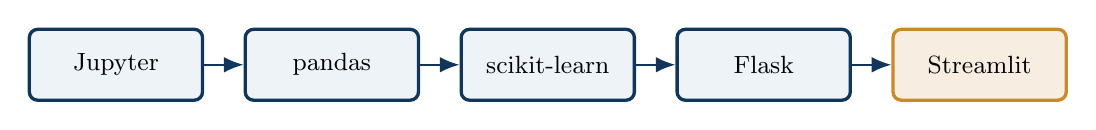
\begin{tikzpicture}[node distance=0.5cm and 0.5cm]
\node[flowbox] (jupyter) {Jupyter};
\node[flowbox, right=of jupyter] (pandas) {pandas};
\node[flowbox, right=of pandas] (sk) {scikit-learn};
\node[flowbox, right=of sk] (flask) {Flask};
\node[accentbox, right=of flask] (st) {Streamlit};
\foreach \a/\b in {jupyter/pandas,pandas/sk,sk/flask,flask/st} {
  \draw[arrow] (\a) -- (\b);
}
\end{tikzpicture}
\vspace{0.6em}
\begin{itemize}
\item Explore and teach in Jupyter, manipulate tables in pandas, model with scikit-learn, serve with Flask, and put an interface in front of it with Streamlit.
\item Every one of these already appears in this repository, not only in slides.
\end{itemize}
\coursefooter
\end{frame}

\begin{frame}{What each tool is actually for}
\begin{tabularx}{\textwidth}{>{\bfseries}l X}
Tool & Job \\
\toprule
Jupyter & Interactive notebooks for exploration, teaching, and narrated analysis. \\
pandas & Loading, inspecting, and reshaping tabular data. \\
scikit-learn & Preprocessing, training, evaluating, and persisting classical ML models. \\
Flask & A lightweight web framework to expose predictions as an API. \\
Streamlit & A rapid way to turn a Python script into an interactive dashboard. \\
\bottomrule
\end{tabularx}
\coursefooter
\end{frame}

\begin{frame}[fragile]{Python you will recognize by the end of this class}
\begin{lstlisting}[style=coursepython]
import streamlit as st

st.set_page_config(
    page_title="440MI - Machine Learning Dashboard",
    page_icon=":robot_face:",
    layout="wide",
    initial_sidebar_state="expanded"
)

st.title("Machine Learning Streamlit Hub")
\end{lstlisting}
\begin{itemize}
\item This is the opening of `streamlit/Main.py`, the entry point of the course's dashboard.
\item Nothing here is exotic: an import, a function call with keyword arguments, and a method call --- core Python syntax we build up starting next class.
\end{itemize}
\coursefooter
\end{frame}

\begin{frame}{Where the toolchain already lives in this repository}
\repoactivity{
\begin{itemize}
\item `requirements.txt` pins pandas, scikit-learn, matplotlib, seaborn, Flask, and lists streamlit and numpy among the project dependencies.
\item `notebooks/` holds the Jupyter material we will use for EDA and model training.
\item `streamlit/Main.py` and `streamlit/pages/` are the dashboards the fraud case will run through.
\item `streamlit/modeling.py` trains and pickles the fraud model students will later serve and inspect.
\end{itemize}
}
\coursefooter
\end{frame}

\begin{frame}{Setting up for this course}
\begin{enumerate}
\item Install Python (3.x) and a package manager, or use a distribution that bundles both.
\item Create an isolated environment for the course so package versions do not collide with other projects.
\item Install the packages listed in `requirements.txt`.
\item Confirm Jupyter starts and a notebook in `notebooks/` runs top to bottom.
\end{enumerate}
\coursefooter
\end{frame}

\begin{frame}{Questions you should be able to answer after Class 2}
\begin{itemize}
\item Why is Python described as interpreted, high-level, and object-oriented, and what does each word actually change?
\item What is the practical trade-off between compiled and interpreted execution?
\item Name one job each of Jupyter, pandas, scikit-learn, Flask, and Streamlit does in this course.
\item Where in this repository does each of those five tools already appear?
\end{itemize}
\coursefooter
\end{frame}

\begin{frame}{Discussion prompt}
\begin{block}{Question}
If Python is slower per instruction than a compiled language, why does it dominate data-driven engineering rather than losing out on performance grounds?
\end{block}
\begin{itemize}
\item Pushes students to separate developer productivity from raw execution speed.
\item Sets up the idea that critical inner loops (NumPy, scikit-learn) are themselves compiled, while Python orchestrates them.
\end{itemize}
\coursefooter
\end{frame}

\begin{frame}{Papers and materials}
\readinglist{
\href{https://jupyter.org/install}{Jupyter install guide};\
\href{https://pandas.pydata.org/docs/}{pandas documentation};\
\href{https://scikit-learn.org/stable/}{scikit-learn documentation};\
\href{https://flask.palletsprojects.com/en/stable/}{Flask documentation};\
\href{https://docs.streamlit.io/get-started}{Get started with Streamlit}.
}
\coursefooter
\end{frame}

\classclosingframe
{\begin{itemize}
\item Python is interpreted, high-level, general-purpose, and object-oriented --- a deliberate combination, not an accident.
\item The trade-off of interpreted execution is worth it for the iteration speed that data-driven work needs.
\item Jupyter, pandas, scikit-learn, Flask, and Streamlit already exist in this repository and will reappear all semester.
\end{itemize}}
{Before writing a line of your own project code, confirm your environment can run the notebooks and dashboards already in this repo.}
{Class 3 starts writing real Python: variables, types, and the small syntax rules every later script depends on.}
{Every tool tour eventually turns into code we read line by line --- that starts next class.}

\end{document}
